\section{Use Case Definitions}\label{sec:use-case-definitions}
Before proceeding further, we formally outline the use cases this project aims to address.
We will describe our use case diagram displayed in figure~\ref{fig:usecases}.

\begin{figure}[!htbp]
    \centering
    \caption{Example of a MLOps pipeline define within Airflow}
    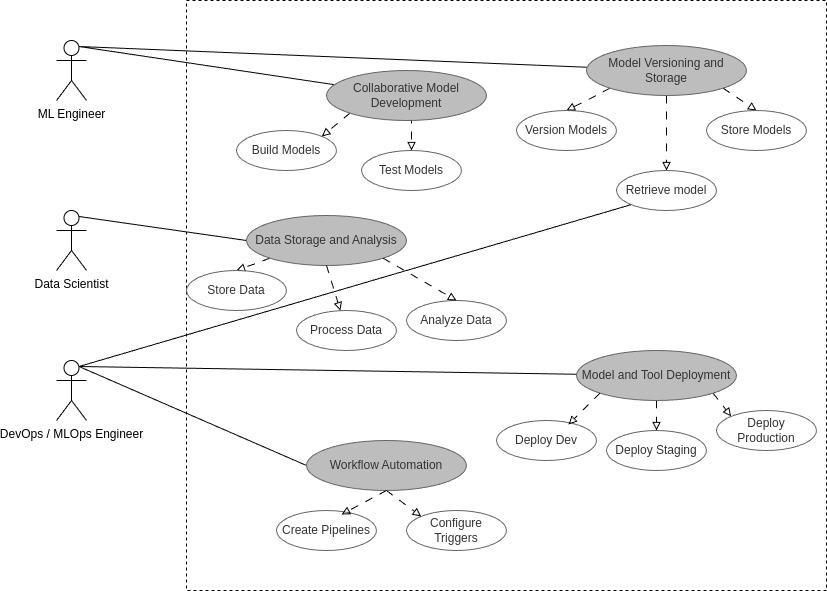
\includegraphics[scale=0.5]{images/project/usecases}
    \label{fig:usecases}
\end{figure}

\subsection{Collaborative Model Development}\label{subsec:collaborative-model-development}
The platform must provide the necessary tools and infrastructure to enable development teams to collaboratively build,
test, and deploy models across segregated environments.

\subsection{Data Storage and Analysis}\label{subsec:data-storage-and-analysis}
A robust system for storing, processing, and analyzing data is required to support model training and evaluation.

\subsection{Model Versioning and Storage}\label{subsec:model-versioning-and-storage}
The solution must include a structured approach to versioning, storing, and retrieving trained models efficiently.

\subsection{Model and Tool Deployment}\label{subsec:model-and-tool-deployment}
The system must support seamless deployment of models and associated tooling across environments—from local development
setups to production—with minimal friction.

\subsection{Workflow Automation}\label{subsec:workflow-automation}
To enhance operational maturity, we prioritize automating repetitive tasks in the workflow.
This will be achieved through well-defined pipelines and triggers, informed by our state-of-the-art review.